\documentclass{article}
\usepackage[utf8]{inputenc}
\usepackage{graphicx}

\title{Anomaly detection in financial data}
\author{Anar Sultani, Daniel Grimm, Gayrat Rakhimov,\\ Zhang Yinghong, Suchith Shetty}
\date{December 2020}

\begin{document}

\maketitle

\section{Introduction}

This project is implementation of anomaly detection on financial data.

\subsection{Datasets}

2 data sets are used:
\begin{itemize}
    \item balance\_hist\_anon.csv - account balance states for certain time periods. It contains 6427316 rows of data.
    It contains 6 columns:
    \begin{enumerate}
    \item EBIZ\_BALANCE\_ID - unique id for each account balance state
    \item VALID\_FROM - the time from which account balance is valid
    \item VALID\_TO - the time till which account balance is valid
    \item GIRONUMBER - account number
    \item AMOUNT - account balance
    \item CURRENCY - currency of account balance
    \end{enumerate}
    \item eurofxref-hist.csv - contains currency exchange rates. It is provided by European Central Bank\cite{ecb} and the base currency is Euro. The following currencies are used:
\begin{itemize}
    \item BGN - Bulgarian lev
    \item CHF - Swiss franc
    \item CZK - Czech krona
    \item EUR - Euro
    \item GBP - Great Britain pound
    \item HRK - Croatian kuna
    \item HUF - Hungarian forint
    \item PLN - Poland zloty
    \item RON - Romanian leu
    \item SEK - Swedish krona
    \item USD - United States dollar
\end{itemize}
\end{itemize}

\newpage
\section{Overall system architecture}
\subsection{System architecture}

\begin{figure}[h!]
\centering
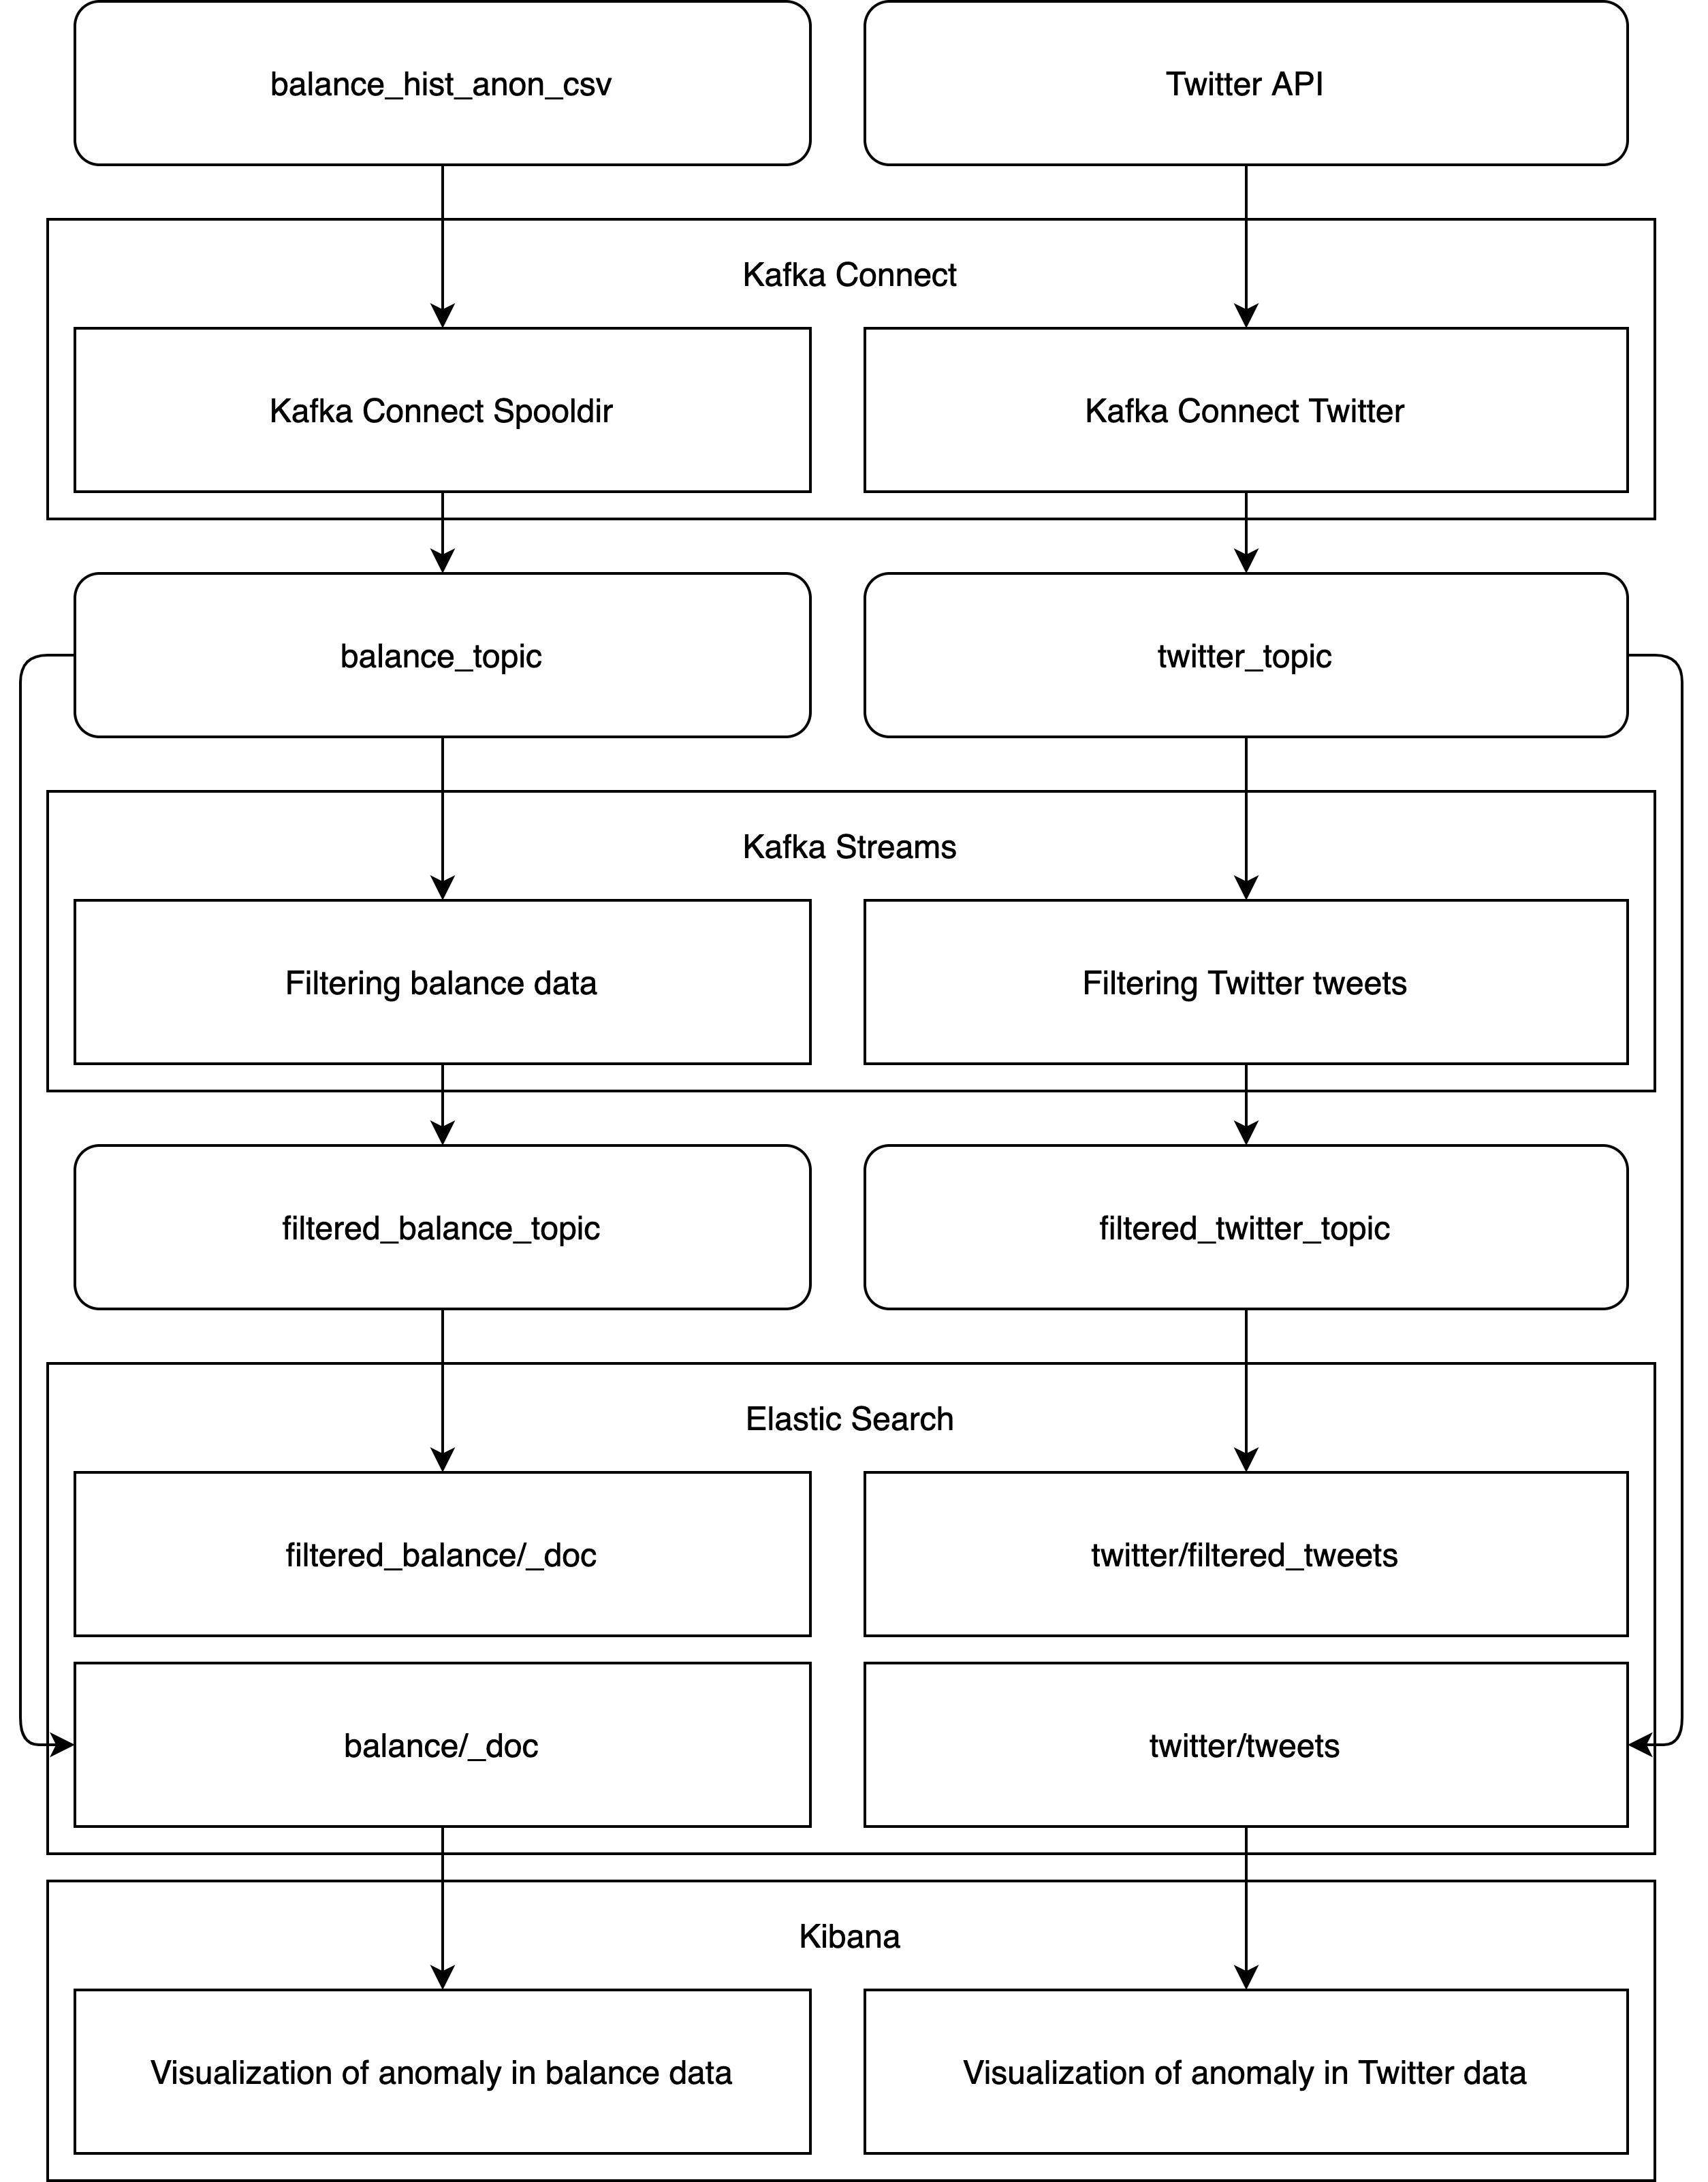
\includegraphics[scale=0.115]{architecture.png}
\caption{System architecture}
\label{fig:universe}
\end{figure}

\newpage
\subsection{Jupyter Notebook}
\subsubsection{Modifying balance data}

Jupyter Notebook was used to understand balance data and rename first column to 'id'. For debugging purposes, it saves part of data (for example, first 10000 rows).

\subsubsection{Modifying exchange rates data}

Initially 'eurofxref-hist.csv' contains exchange rates for 42 currencies from 04.01.1999 till 09.12.2020. According to balance data, only exchange rates for 10 currencies from 02.01.2017 till 09.12.2020 is used. It is important to note that this data set does not contain exchange rates RSD (Serbian dinar).

\subsection{Kafka Connect}

Kafka Connect connector called Spool Dir was used to read 'balance.csv' into the stream 'balance\_topic'. It reads CSV file and converts into JSON format according to the given schema. JSON data is sent to 'balance\_topic'. Batch size is 1000 per batch.

\subsection{Kafka Streams}

\subsubsection{Merging balance data with exchange rates data}

Exchange rates data is read from 'exchange.csv' into HashMap. It is used to update balance data from 'balance\_topic'. For example, when exchange rate is 1 EUR=1.1 USD and account balance 1100 USD is replaced by 1000 EUR.

\subsubsection{Filtering balance data}

First filtering is made on account balance difference. For this purpose, previous balance amount is persisted by account number. When next account balance state is received, difference is calculated and if the difference is more than predefined limit, it is considered as anomalous. For example, previous balance for the account is 5000 EUR and the current balance is 3000 EUR, the difference is 2000 EUR and it is more than 1000 EUR. This is considered as anomalous and sent to 'filtered\_balance\_topic'.

\section{Experiments}

\subsection{Merging 2 streams}

It was tried to merge the balance data and currency exchange data streams into one using Kafka Streams. However, during the implementation of this idea, several problems were faced. For example, the way how to synchronize daily exchange rates with balance data on the given date was not found. Primitive merging of two streams caused the following problem: the balance data is received before exchange rate data for specific day and balance data could not be updated. For this reason, exchange rate data was read directly from file without creating stream.

\subsection{Twitter API}

It was tried to use Twitter tweets feed to help find anomalies on balance data. For example, tweets with keyword "HUF/USD", "HUF/EUR", "Economy of Hungary". However, the meaningful use case of tweets feeds was not found and it was decided to not to use them.

\subsection{Remote ElasticSearch server}

Twitter all tweets and filtered tweets are stored in remote ElasticSearch server called Bonsai. It was found out that it is convenient way to set up ElasticSearch server in short time. However, according to the project requirements balance data should not be stored in third party storage and that's why it was decided to use ElasticSearch on personal computer. 

\section{Description of duties performed by project team members}

\subsection{Anar Sultani}

\subsection{Daniel Grimm}

\subsection{Gayrat Rakhimov}

\begin{itemize}
    \item data preprocessing on Jupyter Notebook: modifying balance and exchange rates data
    \item setting up Kafka Connect to read balance data into 'balance\_topic' stream
    \item reading Twitter tweets feed from Twitter API
    \item merging balance data and exchange data
    \item filtering balance data according to balance differences
    \item setting up remote ElasticSearch server and storing Tweeter tweets there
    \item code repository management on Github: creating repository, reviewing pull requests and access management
    \item participating in project team's meetings
    \item writing report
    \item preparing presentation material
\end{itemize}

\subsection{Zhang Yinghong}

\subsection{Suchith Shetty}

\section{References}

\begin{thebibliography}{9}

\bibitem{ecb} 
European Central Bank. (2020). Euro Foreign Exchange Reference Rates. \url{www.ecb.europa.eu/stats/eurofxref/eurofxref-hist.zip?53a6f7cba144c040b7a2a4a8242d1431}.

\end{thebibliography}

\end{document}
